% !TeX spellcheck = en_US
% !TeX root = ./0_article.tex

\section{Practicing BBI in a better way}
	\IEEEPARstart{T}{his} section is dedicated in presenting BBI platforms and the various improvements which can be brought to increase experiments repeatability and reliability.
	\subsection{BBI platforms in the state of the art}
		In the first place, let us analyze, from a theoretical perspective, a typical BBI platform, such as the one found in the state of the art.
		To do so, we created simple platform models highlighting the major limiting factors of such platforms.
		% !TeX spellcheck = en_US
% !TeX root = ./0_article.tex

\begin{figure}[h]
	\centering
	\subfloat[][Typical]{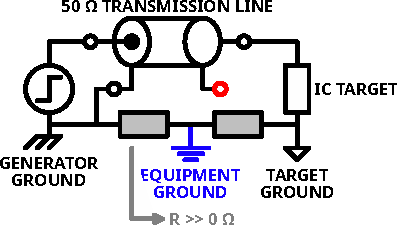
\includegraphics[width=0.5\columnwidth]{./figures/state-of-the-art-platform.pdf}}
	\subfloat[][Improved]{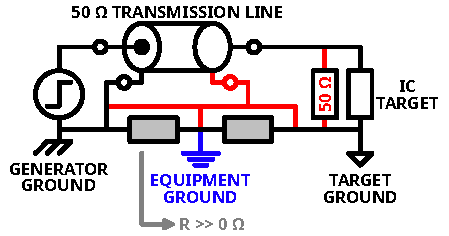
\includegraphics[width=0.5\columnwidth]{./figures/s-bbi-better.pdf}}
	\caption{Simple models of a typical (a) and an improved (b) BBI setup.}
	\label{bbi_setups}
\end{figure}

		The typical platform model is described in Fig. \ref{bbi_setups}a, and illustrates the main components of a BBI platform, while omitting positioning tables, such as:
		\begin{itemize}
			\item The voltage pulse generator;
			\item The transmission line;
			\item The grounding installation;
			\item The IC target.
		\end{itemize}
		In addition to this, the schematic in Fig. \ref{bbi_setups}a shows some important flaws we are going to address.

		While this is not always the case, fast and high-voltage pulse generators are typically specified to be loaded with a 50 \textOmega\ load, or more generally with a fixed load.
		When performing BBI, the backside of the IC is electrically connected to the generator output.
		Therefore, outside of luck alone, it is very rare that the impedance presented by the IC to the generator perfectly matches the required one.
		It implies that the generator will be, most of the time, out of specifications, and that the conditions will vary depending on the chosen IC, the substrate thickness, and the location of the BBI probe.
		This can lead to issues such as errors in the set-point voltage and pulse width, in addition to ringing in the transmission line.
		This represents a first flaw to the typical approach.

		Then, there is the grounding installation.
		The model presents a non-ideal but simple platform grounding.
		The reference node, used by the oscilloscope and the main computer, is represented in blue and called "equipment ground".
		Ideally, every ground on the platform is connected to this reference node with a very low impedance interconnection.
		However, depending on the hardware used, it may greatly vary from one platform to another.
		In the model, the generator and target grounds are connected to the reference node thanks to vastly imperfect interconnections, whose impedance is significantly greater than zero.
		This mainly lead to set-point errors due to shifts in the voltage pulse amplitude.
		Therefore, it limits the inter-platform repeatability and comparison of BBI experiments.

	\subsection{Our BBI platform}
		As most BBI platforms, our platform is focused on three main pieces of equipment: a voltage pulse generator, a metallic probe (Fig. \ref{bbi_probe}), and a positioning table.
		
		The positioning table we use is an OWIS PS 35 control unit, allowing to drive three motors for free movement in three dimensions.
		The generator model is the AVRK-4-B from the company Avtech Electrosystems Ltd.
		This model is commonly used for EMFI, but is suitable for BBI or any other application requiring fast voltage pulses, and its specifications are the following:
		\begin{itemize}
			\item Pulse amplitude: \textpm\ [150, 750] V;
			\item Pulse width: [6, 20] ns;
			\item First edge rise/fall time: 4 ns;
			\item Second edge rise/fall time: load dependent;
			\item Recovery time: \textless\ 1 ms;
			\item Propagation delay (PD): 150 ns;
			\item Jitter: \textpm\ 100 ps \textpm\ 0.03 \% of PD;
			\item DC-coupled output;
			\item Loaded with 50 \textOmega.
		\end{itemize}
		% !TeX spellcheck = en_US
% !TeX root = ./0_article.tex

\begin{figure}
	\centering
	\subfloat[][Global view]{\includegraphics[width=0.4\columnwidth]{./figures/sondeBBI_loin_raw.png}}
	\hspace{0.1\columnwidth}
	\subfloat[][Zoomed view]{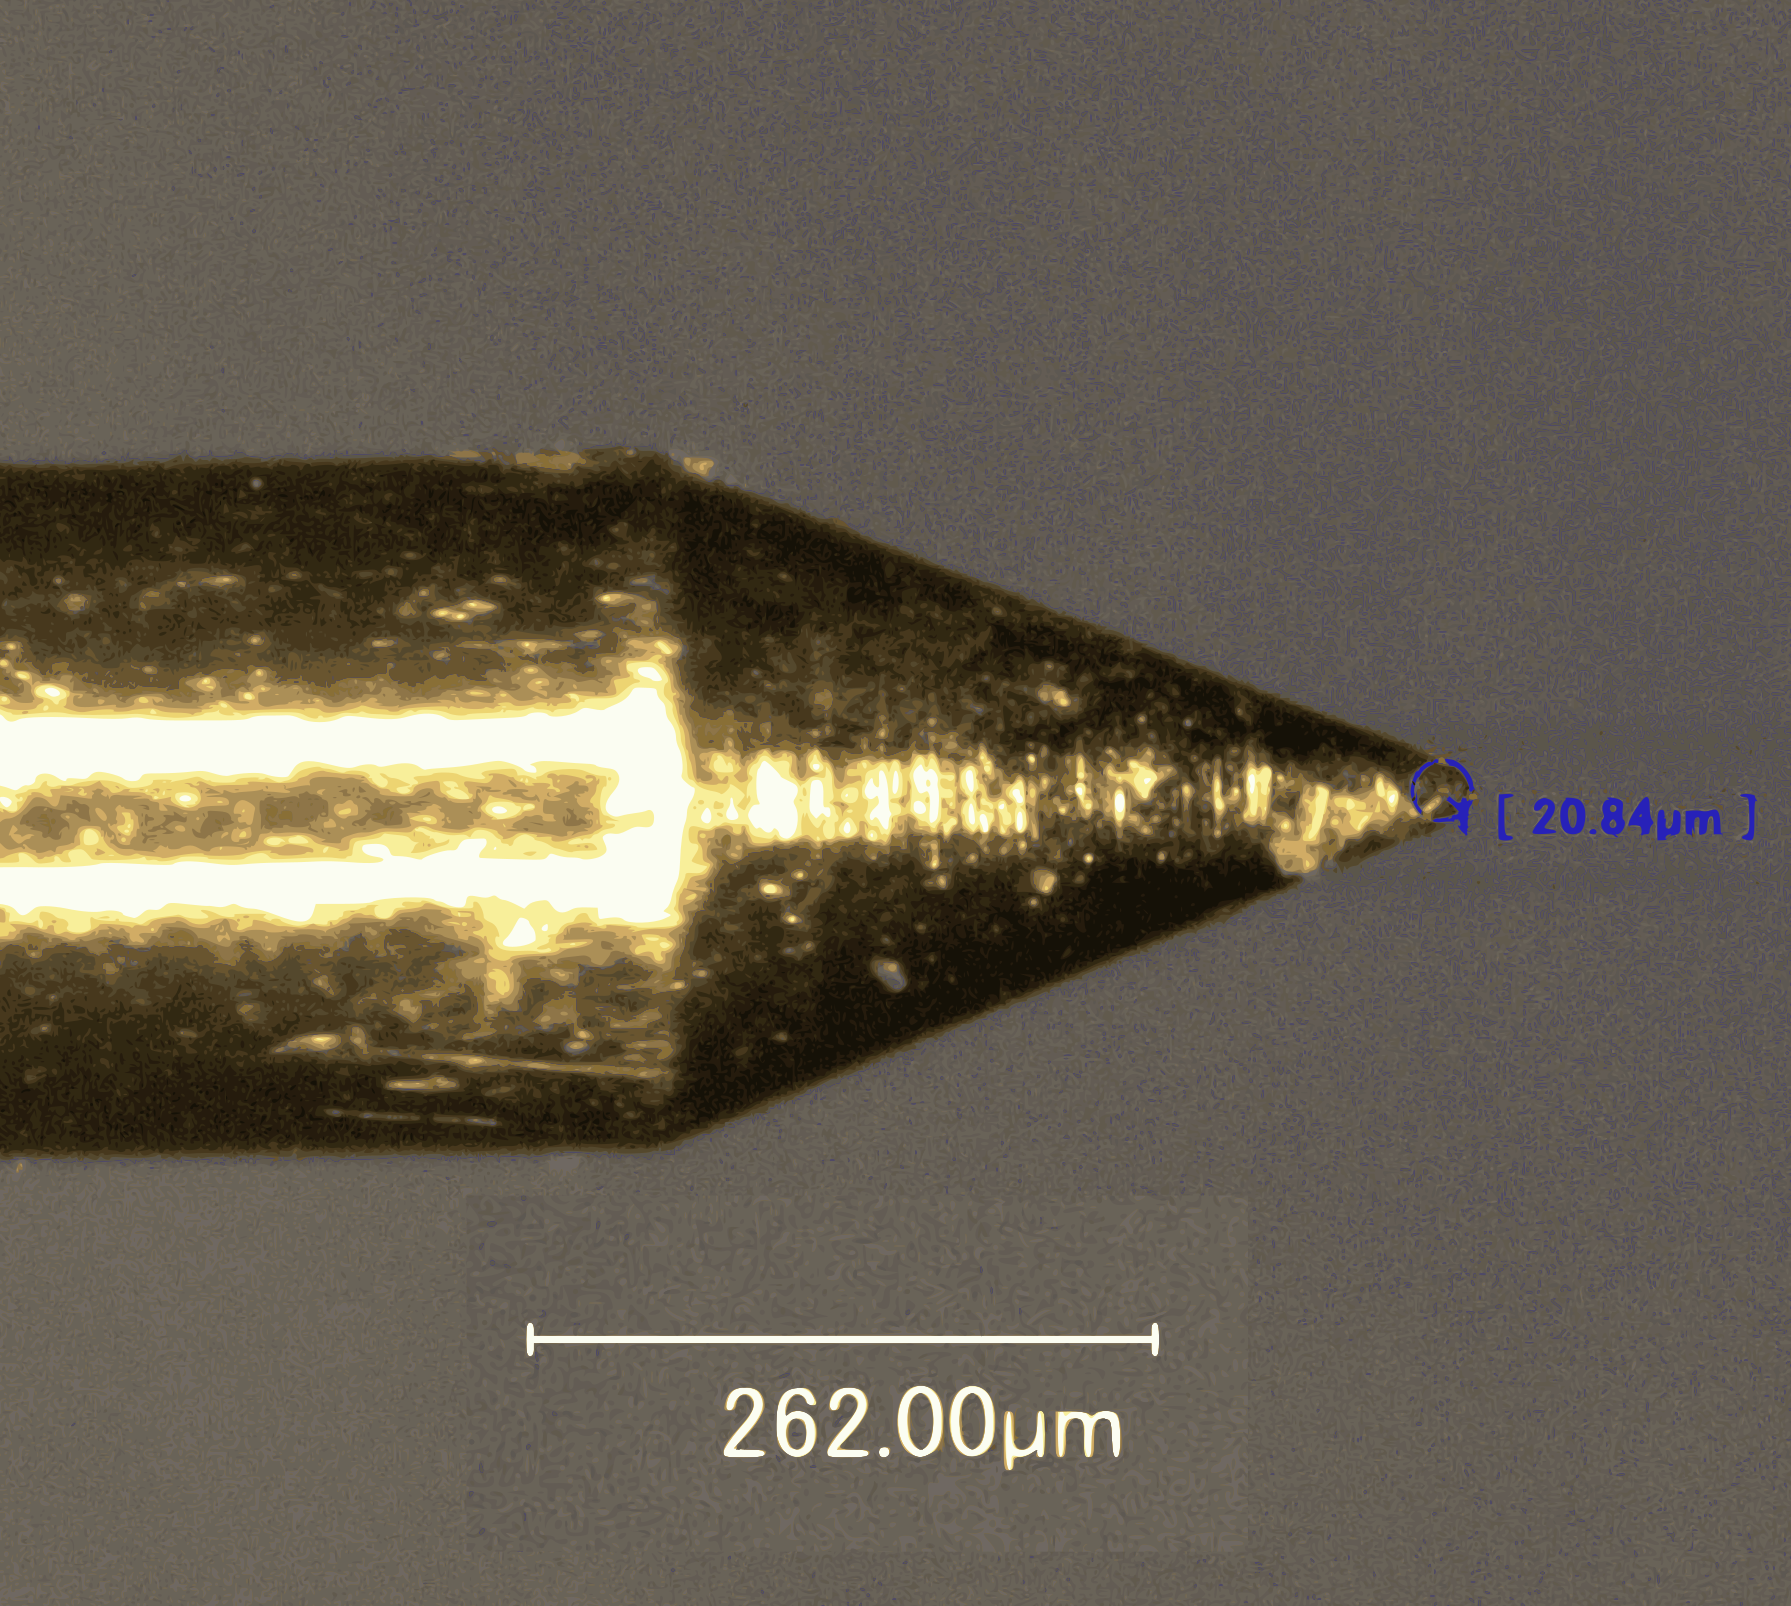
\includegraphics[width=0.4\columnwidth]{./figures/pointeBBI2.png}}
	\caption{Our custom BBI probe.}
	\label{bbi_probe}
\end{figure}
		Eventually, the most distinctive piece of equipment when it comes to BBI is the probe.
%		Probably the most distinctive piece of equipment when it comes top BBI is the probe.
		Some BBI probes can be active, others passive and less expensive.
		However, it is important to keep this piece of equipment relatively cheap as it endures most of the physical strain on the setup, and should be easy to replace or repair.
		Fig. \ref{bbi_probe} shows two pictures of our probe from different angles.
		The one we use is custom-made around three parts:
		\begin{itemize}
			\item A spring-loaded metallic tip, with a 20 \textmu m head diameter;
			\item A SMA connector, where the tip is soldered;
			\item A custom 3D-printed enclosure holding the pieces together and cheap to replace.
		\end{itemize}
		The spring-loaded tip is 17 mm long and has a global diameter of 0.635 mm.
		It is specified for a 1.5 A nominal current, and its electrical resistance measures around 70 m\textOmega.
%		The total cost of the probe is roughly of 20 \texteuro.

	\subsection{The proposed platform enhancements}
		To address the aforementioned limitations, we propose two modifications to generalize the platform and improve  their repeatability.

		First, let us talk about the generator impedance mismatch.
		For this purpose, multiple solutions can be approached.
		The best solution would be to implement an adaptive impedance matching system with active feedback, able to measure in real-time the impedance seen by the generator.
		However, adopting such a method is costly and long to set up in comparison to the next solution.
		Therefore, we propose a much simpler approach.
		Since, most of the time with our platform and targets, the impedance presented by the IC on its backside is in the order of 1 k \textOmega\ \cite{mybbifdtc2023}, approaching the 50 \textOmega\ expected by the generator can be done by connecting a 50 \textOmega\ resistor in parallel to the IC, as shown in the schematic in Fig. \ref{bbi_setups}b.
		
		Then, concerning the platform grounding, the solution is fairly straightforward.
		We propose to choose a reference node, such as the equipment ground in our scenario, and bypass every other ground on the platform with low-impedance interconnections from the previously chosen reference node, as proposed in Fig. \ref{bbi_setups}b.

%		First, let us talk about the improper grounding,
%		Alleviating this issue is fairly straightforward.
%		To do so, we propose to choose a reference, such as the equipment ground, and bypass all the grounds with low-impedance interconnections from this reference, as proposed in red in Fig. \ref{bbi_setups}.b.
%
%		Then, concerning the impedance mismatch of the generator, multiple solutions can be approached.
%		The best solution would be to implement an adaptive impedance matching system with active feedback, able to measure in real-time the impedance seen by the generator.
%		However, adopting such a method is costly and long to set up in comparison to the next solution.
%		Therefore, we propose a much simpler approach.
%		Since, most of the time, the impedance presented by the IC on its backside is in the order of 1 k\textOmega\, approaching the 50 \textOmega\ expected by the generator can be done by connecting in parallel to the IC a 50 \textOmega\ resistor, as it is shown in the schematic in Fig. \ref{bbi_setups}.b.

	\subsection{Platform enhancement validation}
		% !TeX spellcheck = en_US
% !TeX root = ./0_article.tex

\begin{figure}[h]
	\centering
%	\subfloat[][Typical]{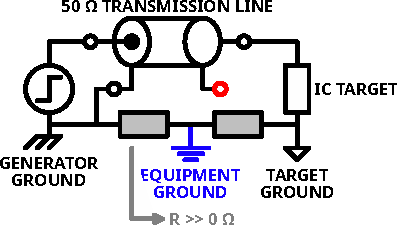
\includegraphics[width=0.5\columnwidth]{./figures/state-of-the-art-platform.pdf}}
%	\subfloat[][Improved]{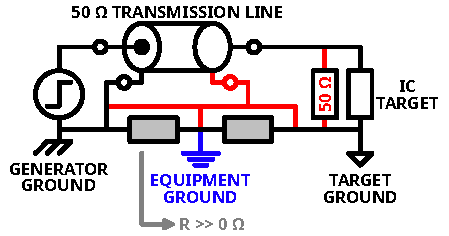
\includegraphics[width=0.5\columnwidth]{./figures/s-bbi-better.pdf}}
	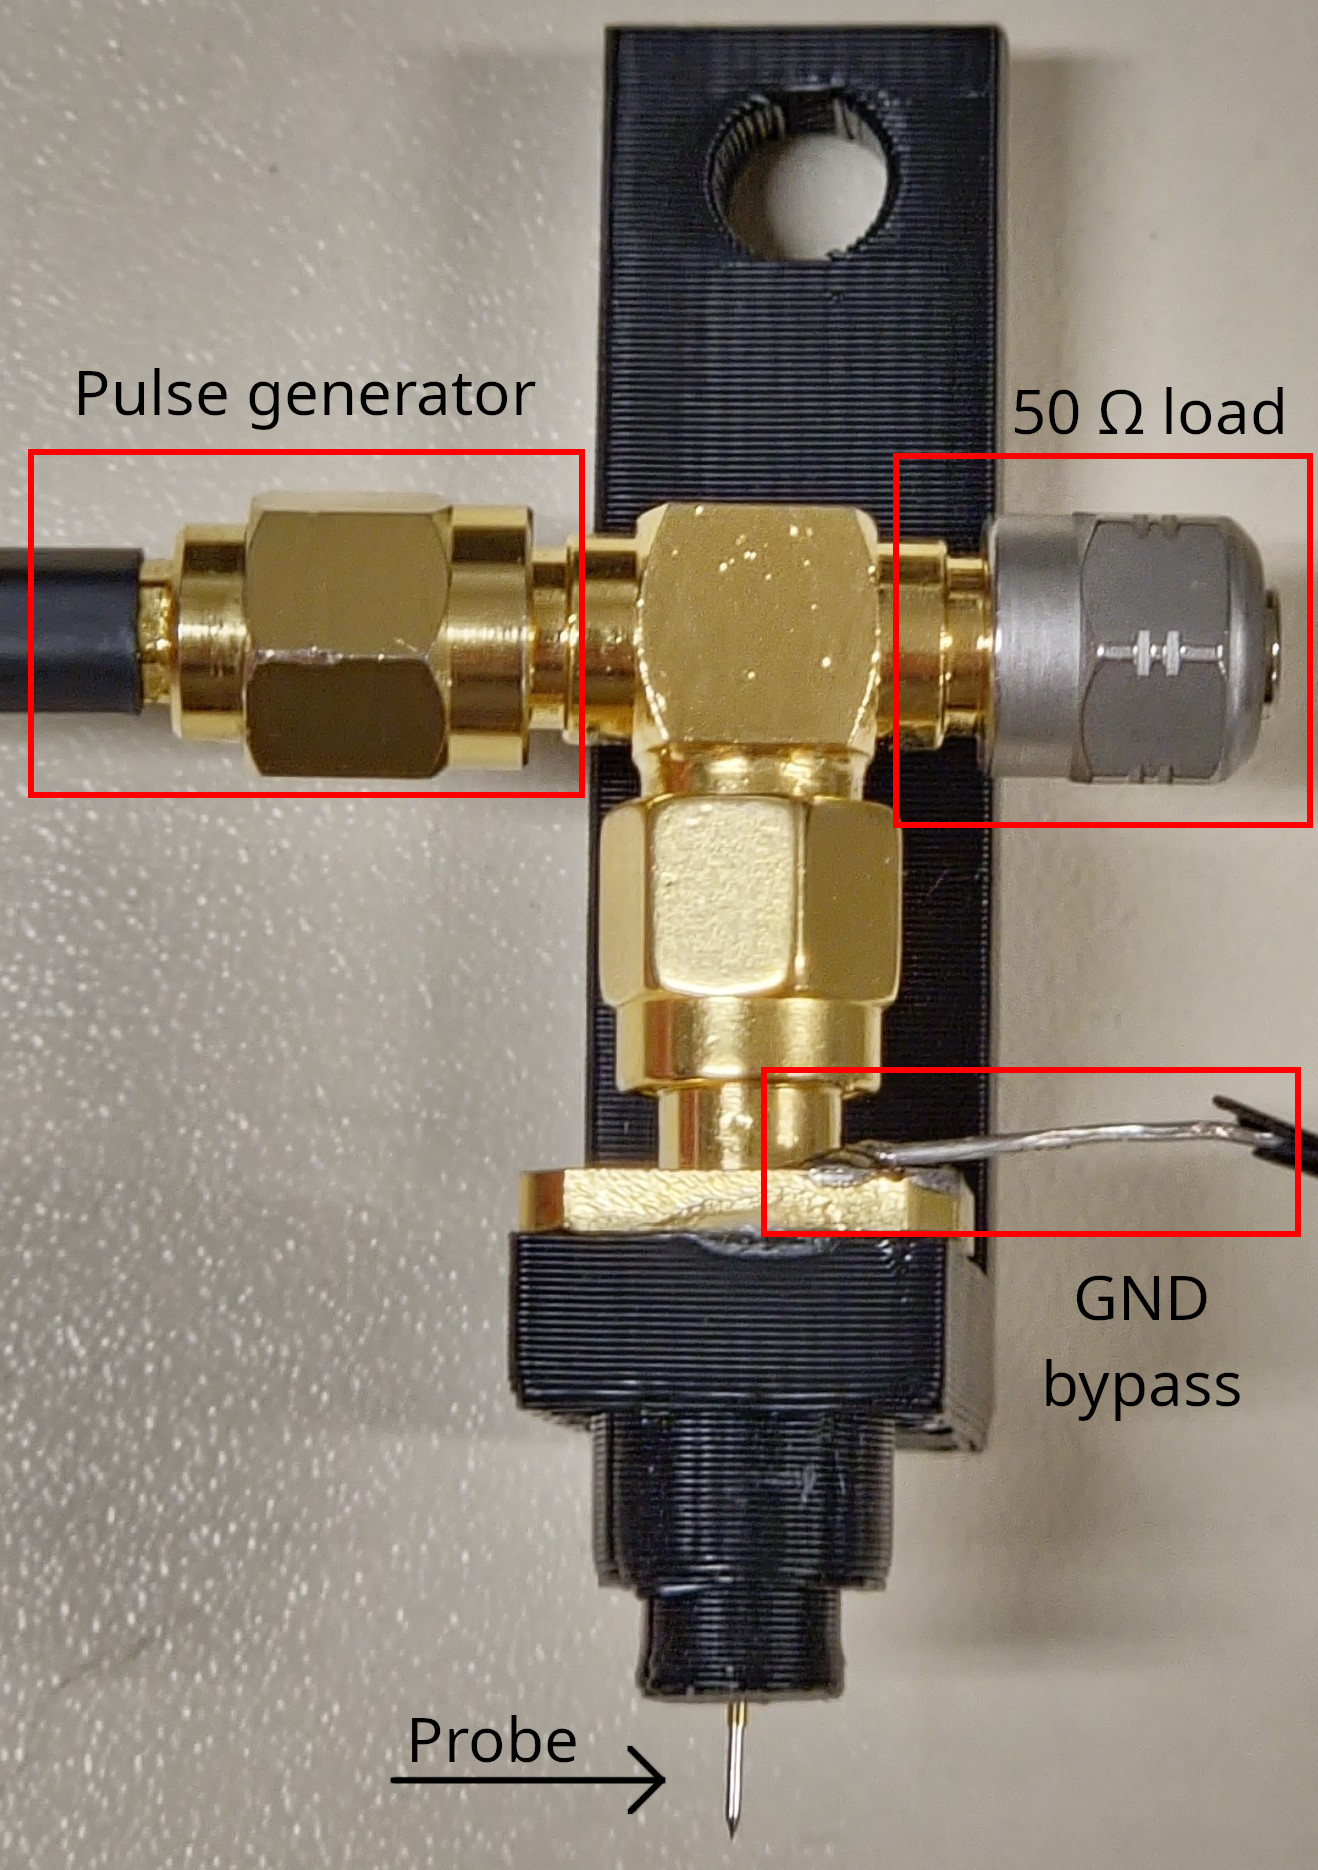
\includegraphics[width=0.40\columnwidth]{./figures/sondeGndSource.jpg}
	\caption{Impedance matching in practice.}
	\label{imp_match_real}
\end{figure}

		Now that we have outlined the platform improvements theoretically, let us analyze their actual impact on our BBI platform.
		The proposed solution concerning the approximate impedance matching and ground bypassing is shown in \mbox{Fig. \ref{imp_match_real}}.
		The picture illustrates the BBI probe with a compensation load connected in parallel. in addition to the probe ground bypass.
		To highlight the practical benefits of these enhancements, let us analyze measured signals extracted from our platform.

		We will compare before and after results and analyze the differences made by these improvements.
		To that end, we set up simple experiments consisting in injecting a voltage pulse into our IC target, measuring the voltage pulse at the probe and the current in the IC.
		% !TeX spellcheck = en_US
% !TeX root = ./0_article.tex

\begin{figure}[h]
	\centering
	%	\subfloat[][Typical]{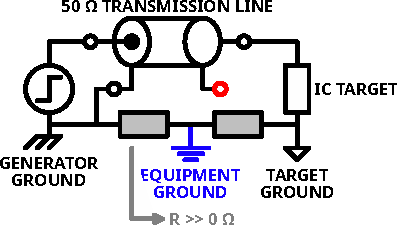
\includegraphics[width=0.5\columnwidth]{./figures/state-of-the-art-platform.pdf}}
	%	\subfloat[][Improved]{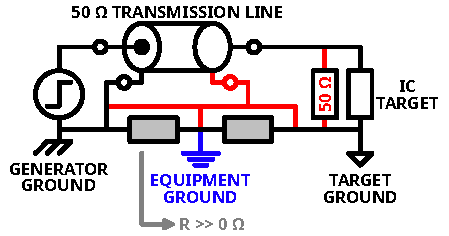
\includegraphics[width=0.5\columnwidth]{./figures/s-bbi-better.pdf}}
	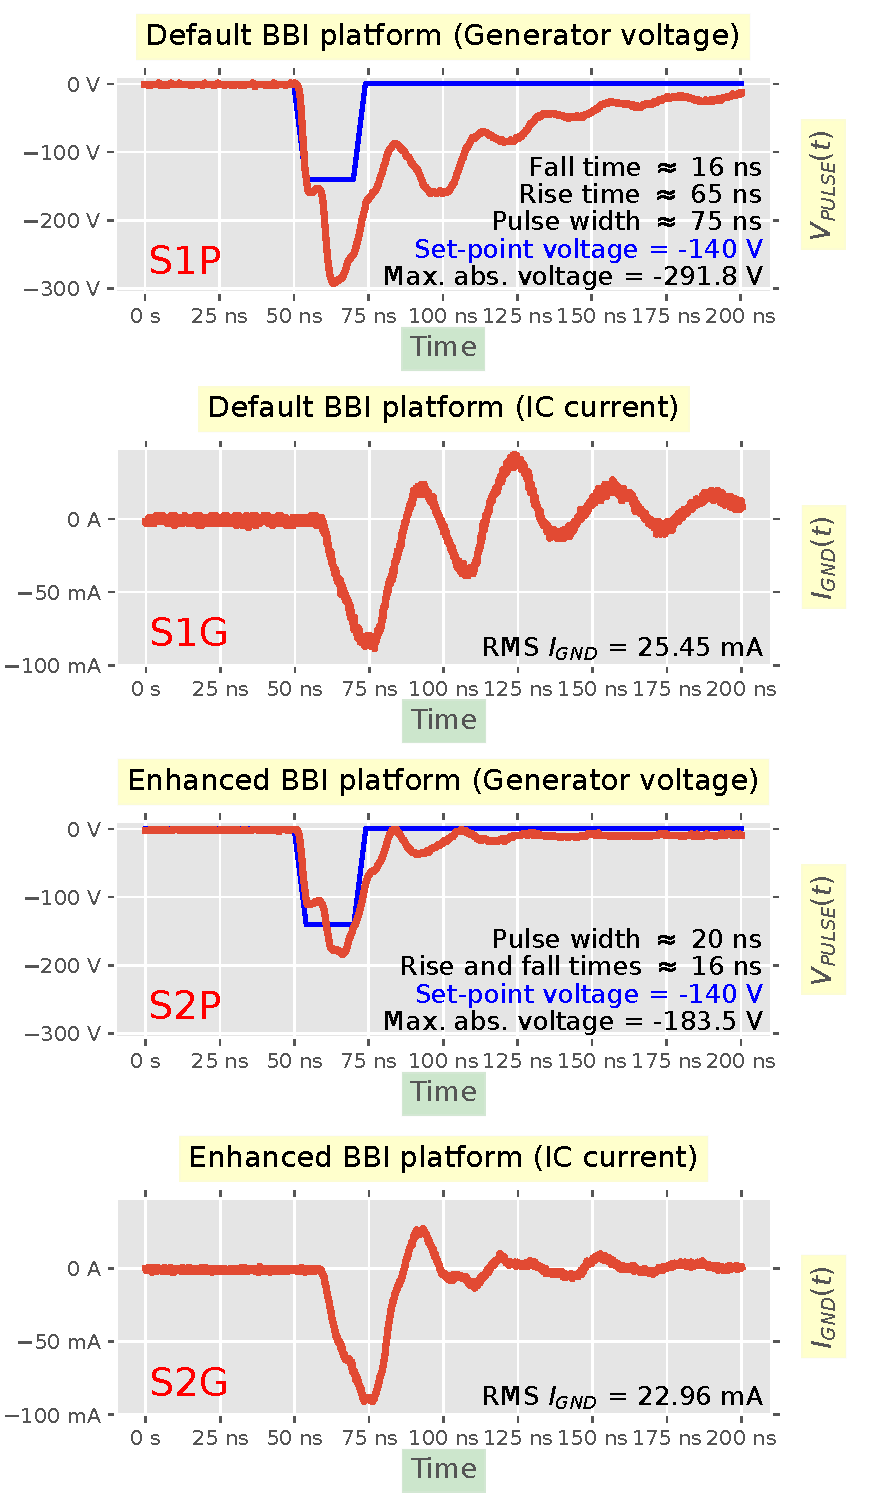
\includegraphics[width=\columnwidth]{./figures/realPulsesComparisons.pdf}
	\caption{Platform improvements in practice}
	\label{actual_imp}
\end{figure}

		Fig. \ref{actual_imp} shows the waveform results from these experiments.
		The figure shows four distinct signals, arranged in the following order:
		\begin{itemize}
			\item S1P: the voltage pulse before improvements;
			\item S1G: the IC ground current before improvements;
			\item S2P: the voltage pulse after improvements;
			\item S2G: the IC ground current after improvements.
		\end{itemize}
%		The figure is split in two main parts, the top row shows the results before the improvements, and the bottom row shows the results after the improvements.
		The experimental conditions are the following:
		\begin{itemize}
			\item Voltage pulse amplitude = -140 V;
			\item Voltage pulse width = 20 ns;
			\item Rise and fall times = 4 ns.
		\end{itemize}

		The waveform S1P shows in blue the ideal waveform according to the generator settings and in red the measured waveform.
		In addition to this are annotated some noteworthy values: such as the set-point voltage of -140 V, the max absolute measured voltage of 292 V, and rise and fall times.
		The first thing to notice here is the obvious undershoot of about -110 \% under the set-point.
		It is far from being desirable when performing fault injection as the voltage amplitude control is of great importance for precision purposes when considering the method effects on the IC \cite{mybbifdtc2023}.
		Furthermore, the pulse width is 275 \% higher than the set-point, measuring 75 ns instead of 20 ns.
		It is an additional issue as it annihilates the accuracy needed in this context, and leads to longer pulses injected into the IC, and therefore energy than required and uncontrollable behavior.
		Additionally, the rise and fall times are also 4 to 16 times higher than expected.
		Eventually, we can notice damped oscillations, an observation of ringing in the transmission line.

		Then, the waveform S1G, associated with the previous one, shows the IC ground current.
		Here, the damped oscillations are more clearly visible, in addition to the much longer than expected pulse duration.
		The RMS value of the injected current measures around 25 mA.

		Afterward, the waveform S2P shows the voltage results with the proposed improvements.
		The voltage pulse amplitude is much closer to the set-point, with an undershoot reduced to -31 \%.
		It is not perfect, but considering the simple nature of the impedance matching method we propose, it was to be expected.
		On another note, the pulse width set-point is perfectly respected.
		However, the rise and fall times are still 4 times higher.
		
		Eventually, when looking at the S2G current waveform, we can remark the ringing reduction, while the amount of transferred energy remains approximately the same.

	\subsection{Platform enhancement application}
		To be able to illustrate further the actual interests of the proposed improvements, we did not only set up electrical measurements, but a complete differential fault attack (DFA).
		Indeed, performing fault injection is mainly used to perform attacks, therefore it makes sense to verify the soundness of the improvements in this context.
		We chose to perform a single bit DFA on our IC target, as the fault criterion is hard to obtain, and therefore it can easily show the interest, or the lack of interest, of performing such improvements to the platform.
		
		The target we used embeds a dedicated cryptographic core, which we set up using an AES on 128 bits.
		We then decided to perform the Giraud's DFA \cite{giraudDfa}, originally described in 2002.
		This attack requires creating single bit faults in one or more bytes on the targeted AES.
		Our target was clocked at 40 MHz thanks to an external 8 MHz crystal, and externally powered with 3.3 V.

		\subsubsection{Preliminary experiments}
			Before setting up the attack, we had to set up preliminary experiments allowing us to find optimal locations on the IC backside where the attack would be performed.
			Indeed, many areas and experimental parameters do not allow observing single-bit faults.
			
			To do so, we created what we call Fault Analysis Mappings (FAM).
			These experiments consist in creating maps of a specific region of the IC, in that case the AES co-processor, and analyzing the IC behavior while performing BBI for a set of various experimental parameters.
			We split the observed behavior into seven cases:
			\begin{itemize}
				\item Correct: the AES responds normally;
				\item Monobit Monobyte fault: a unique bit faulted on a unique byte;
				\item Multibit Monobyte faults: multiple bits faulted on a unique byte;
				\item Monobit Multibyte faults: multiple bytes faulted with a single bit each;
				\item Multibit Multibyte faults: multiple bytes faulted with multiple bits each;
				\item Crash: the circuit did not respond correctly;
				\item Timeout: the circuit did not respond.
			\end{itemize}
			Therefore, as we only need single bit faults, only two cases are valid for the Giraud's DFA.
			To compare the two platforms, we performed a FAM on each one of them, using the following parameters:
			\begin{itemize}
				\item Pulse amplitude: from -150 V to -400 V with -5 V steps;
				\item Pulse width: 4.5 ns;
				\item Pulse delay: 150 ns + 553 ns targeting the penultimate AES round;
				\item Displacement step: 40 mm for the BBI probe over the mapped area.
			\end{itemize}
			Depending on the IC behavior, the experiments can take up to 36 hours.
			The parameters were chosen to minimize the maximum energy transferred into the IC to avoid damaging it as much as possible.
			% !TeX spellcheck = en_US
% !TeX root = ./0_article.tex

\begin{figure}[h]
	\centering
%		\subfloat[][Typical]{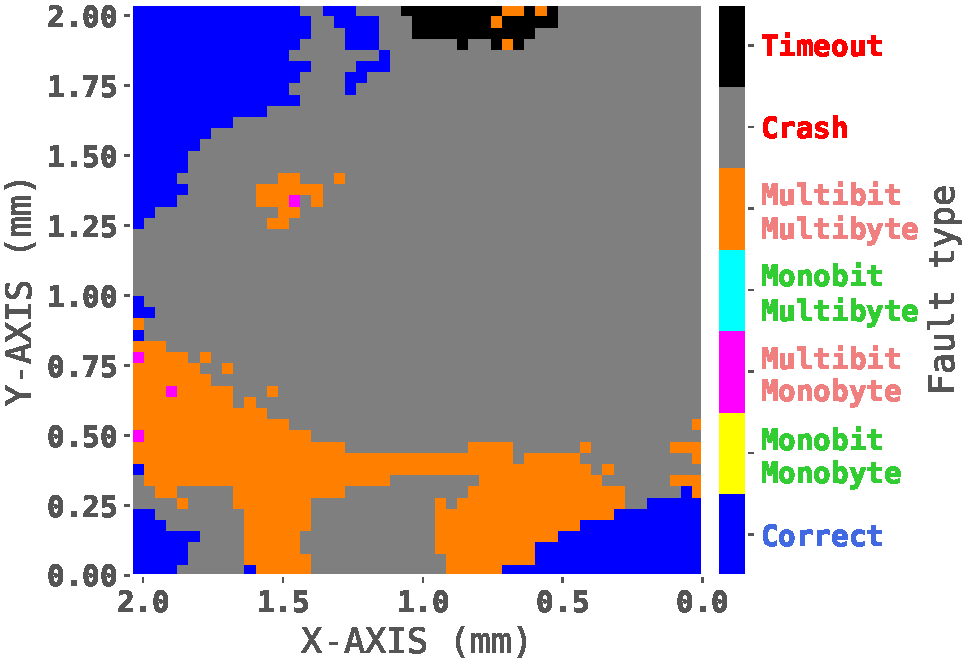
\includegraphics[width=0.5\columnwidth]{./figures/aesFastGndOnly-cropped.pdf}}
%		\subfloat[][Improved]{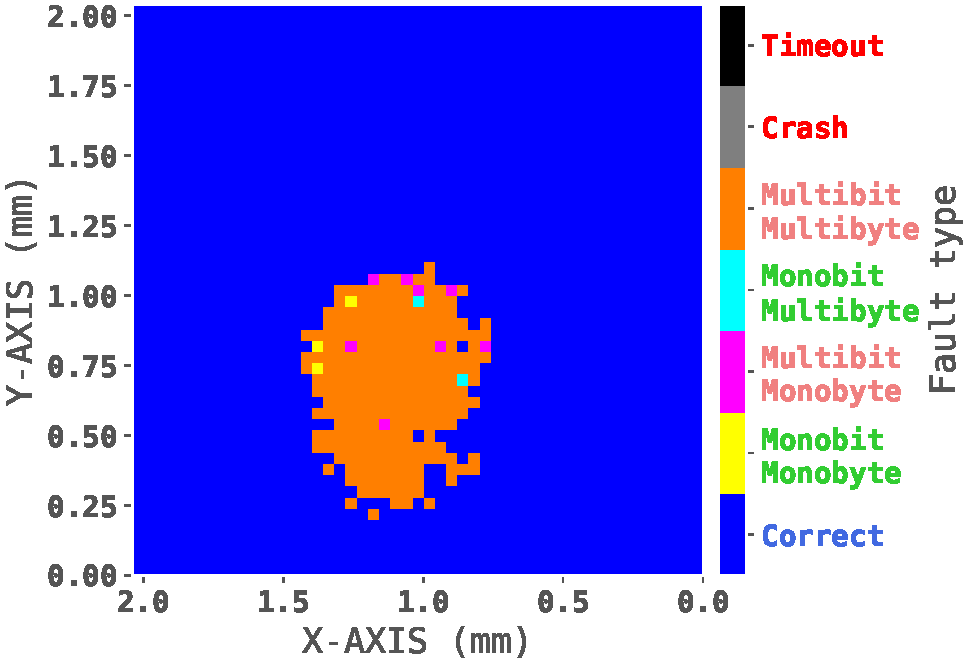
\includegraphics[width=0.5\columnwidth]{./figures/aesFastImpGnd-cropped.pdf}}
		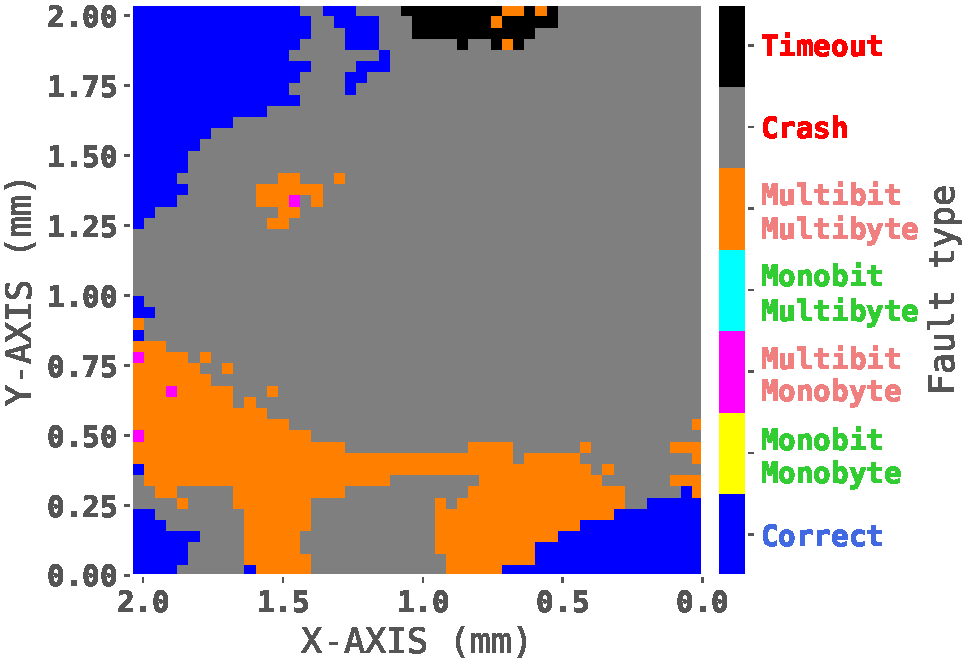
\includegraphics[width=0.995\columnwidth]{./figures/aesFastGndOnly-cropped.pdf}
		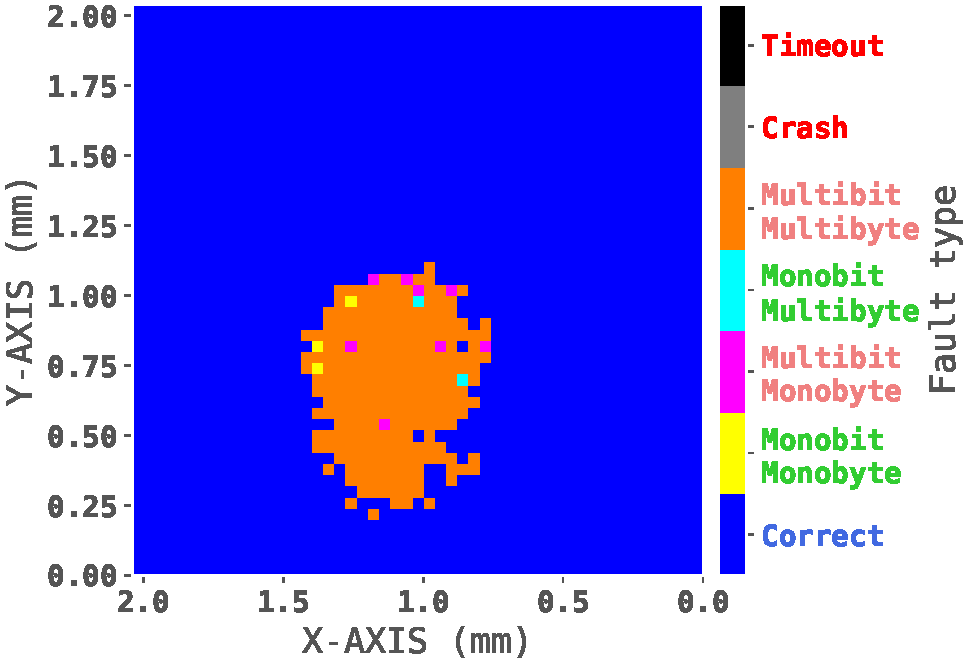
\includegraphics[width=1.0\columnwidth]{./figures/aesFastImpGnd-cropped.pdf}
	\caption{Giraud's attack preliminary FAM}
	\label{giraud_fam}
\end{figure}

			Fig. \ref{giraud_fam} presents the FAM results for both a typical (top) and the improved (bottom) platforms.
			The mapped area encloses a little more than the actual AES location, to be sure to map its entirety.

			Let us look at Fig. \ref{giraud_fam} (top) first.
			What is interesting here is that we can spot numerous locations where the circuit crashed.
			More specifically, they represent 70 \% of the mapped area.
			This behavior is problematic in such an experiment as it cannot lead to any useful data for a DFA.
			We first thought that the experimental parameters were at fault, so we reiterated the experiment using various different sets of parameters, only to observe a majority of crashed locations, while never observing any single bit fault.
%			Despite trying various experimental parameters, we could not observe single bit faults using this setup.
%			However, multibit multibyte faults were easily observed, which was to be expected as they are easy to perform without much effort.

			Then, let us discuss Fig. \ref{giraud_fam} (bottom).
			The first interesting thing to remark here is the total absence of IC crash.
			It is a desirable behavior as it indicates that we did not set a too high voltage or a too long pulse.
			Then, concerning single bit faults, we can spot five locations.
			It is a good sign for a preliminary experiment as it indicates the feasibility of such faults without much effort.
			However, it does not mean that we can perform the attack on one location with one set of parameters.
			It rather means that we can use these locations as good starting points to perform the DFA.

		\subsubsection{DFA results}
			To perform the DFA, we focused on the five previously found monobit locations above the AES core.
			Then, for each location, we used the following parameters:
			\begin{itemize}
				\item Voltage ranging from -300 V to -600 V;
				\item Pulse width ranging from 4.5 ns to 5.5 ns;
				\item Injection delay ranging from \textpm 10 ns around the penultimate AES round.
			\end{itemize}
			For each set of experimental parameters, we had to set some limits when trying to inject faults.
			Indeed, it is required to create a finite and of reasonable length experiment.
			The first limit consists in trying to retrieve a maximum of 100 single bit faults.
			We have chosen this value as it is far more than what is suggested by Giraud's DFA \cite{giraudDfa} description.
			However, if reaching this limit can be easy on some sets of location and parameters, on others, it is almost impossible.
			Therefore, we have set another limit of 10000 trials to achieve the previous goal.
			% !TeX spellcheck = en_US
% !TeX root = ./0_article.tex

\begin{table*}[ht]
	\centering
	\begin{tabularx}{\textwidth}{XXXXXXXXXXXXXXXXX}
		\#B & 0 & 1 & 2 & 3 & 4 & 5 & 6 & 7 & 8 & 9 & 10 & 11 & 12 & 13 & 14 & 15 \\ \hline
		K10 & 0xFF & 0x1F & \cellcolor{red!25}0x42 & 0xE8 & 0xEF & \cellcolor{red!25}0x44 & 0xA5 & 0x6A & 0xCA & 0xE7 & 0x55 & 0x3C & 0xFD & 0x65 & 0x39 & 0x26 \\
		KEY & 0x01 & 0x23 & 0x45 & 0x67 & 0x89 & 0xAB & 0xCD & 0xEF & 0xDE & 0xAD & 0xBE & 0xEF & 0x12 & 0x34 & 0x43 & 0x21
	\end{tabularx}
	\caption{Giraud DFA}
	\label{table_giraud}
\end{table*}

			Thanks to this experiment, we retrieved, using the five previously identified locations, 14 bytes out of 16 of the AES K10 key, which is directly linked to the secret key in an AES-128 bits implementation, as shown in Table \ref{table_giraud}.
			We could not retrieve with the Giraud's DFA the bytes number 2 and 5, which are located in the red cells in the previous table.
			To retrieve the key in its entirety, we performed a brute force method consisting in calculating every possibility for the remaining two bytes.
			Considering a slow laptop being able to compute approximately $10 \cdot 10^3$ AES encryptions per second, and the 16 remaining bits representing 65536 combinations, we decided to blindly calculate every combination.
			This calculation represents around 6.5 seconds of total computation time, and the results are shown in Table \ref{table_giraud}.
			This experiment demonstrates the soundness of the proposed platform enhancements in terms of end user applications, i.e. a differential fault attack.

%	Three main flaws lie in the platform in its current state:
%	\begin{itemize}
%		\item The pulse generator
%	\end{itemize}
